% !TeX spellcheck = en_GB
% !TeX spellcheck = en_US 
\chapter{Theoretical Background}

In this chapter we will present all the theoretical background necessary for the development of this project, from the theory and creation of the He droplets to the physics behind the plasma and coulomb explosion process to the detection techniques. In order to guide the reader in an organised way, the chapters are organized in a way that follow the processes necessaries to the performance of the experiment. this means that all the chapters explained in here occurrence in the same order during the experiment.


\section{Helium Nanodroplets}

The combination of cryogenic matrix isolation, discovered in 1954 \cite{whittle_matrix_1954}, and the now well defined properties of Helium ($He$), specially its superfluidity face discovered in 1937 by \textit{Kapitza et. all}            \cite{kapitza_viscosity_1938}, have as consequence one of the most powerful and flexible tool in physics, the helium nanodroplets.
Helium nanodrops  have unique properties that makes it  very suitable for the cluster and nanophysics experiments in the last decades. For example, they do not exhibit any optical transitions in the entire infrared, visible and ultraviolet range. They can readily pick up atoms and molecules and  form complexes from the species embedded in their interiors, or on their surfaces and act as a ideal matrix for atom, molecules and clusters isolation. \cite{stienkemeier_spectroscopy_2006}\cite{toennies_superfluid_2004}.
The size of a He cluster can go from of a few thousands up to $10^{8}$ of atoms, and reach temperatures at   ultra cold temperature regime (close to 0.37$K$ \cite{toennies_spectroscopy_1998})\cite{enss_low-temperature_2005}.
Two main advantages of this  cooling properties arise. First,  dopants in the He nanodroplet are set to their absolute vibronic ground states, avoiding all other possible espectra and stablishing the cluster in a specific state, more important, the fast cooling helps to the formation of isomers that are difficult or impossible to generate with other methods \cite{nauta_nonequilibrium_1999}. Second, because the superfluid fase of the He nanodroplets\cite{grebenev_superfluidity_1998}, the bond between dopants and He is weak. Therefore, in contrast to spectroscopy in other matrices with higher temperatures, the optical transitions of many dopants are barely influenced by the He matrix \cite{toennies_superfluid_2004}. 
The theory of  He superfluidity will not be part of this section, this imformation is well documented in other sources, and here we are based on ref.\cite{enss_low-temperature_2005} where all theory is well presented to the reader. In the next section we will dedicate a bigger effort on explain the theoretical and technical background of the He nanodroplets creation as well as the physical and technical process to doped it. 

\subsection{He Nano droplets production}

At room temperature, helium is a light inert gas. It is odorless, colorless, tasteless, and after hydrogen, the second most abundant element in the universe.  \cite{enss_low-temperature_2005}. It have a simple 2 atoms structure, exhibing numerous exotic phenomena whose theoretical descriptions are rather complex in many cases, i.e it characteristics of  a quantum fluid. From helium exist  two stable isotopes $^{3}He$ and $^{4}He$.  $^{4}He$ has two electrons, two protons and two neutrons, no nuclear spin and no total spin, pertaining to the bosonic family, while $^{3}He$ with only one neutron has a spin of $I = 1/2$ and belongs to the fermions \cite{atkins_liquid_2014}.

The bosonic state $_{4}He$ is specially of interest, at  temperature T$\leqslant$2.8K and under normal pressure has a phase transition from "normal liquid" He-I to super liquid He-II \cite{swenson_liquid-solid_1950}, in which the helium can be described by a Bose-Einstein condensation. Even the fermionic $^{3}He$ exhibits this phase transition at T$\leqslant 0.03K$ \cite{halperin_properties_1978}.

The superfluidity of $He-II$, at temperatures close to absolute zero, brings with it some unique features. The essential Properties for this include an almost disappearing viscosity in the superfluid phase, weak interaction, very efficient cooling, and the Transparency for electromagnetic radiation up to wavelengths in vacuum ultraviolets (VUV) Spectral range \cite{enss_low-temperature_2005}. Helium has therefore in the complete visible spectrum no transitions from the ground state. Through the noble gas configuration, helium has a spherically symmetrical electron distribution \cite{lewis_helium_2014}, it can hardly be polarized and is the least reactive of all the elements.

\subsubsection{Helium Droplets}

The production He droplets had to overcome first one principal problem, its liquefaction. At the end  of 19th century many gases were liquefied for the first time by applying pressure at room temperature. However, for He and hydrogen, this method was not successful. In 1922 Kamerlingh Onnes reached temperatures below $1K$ by reducing the vapor pressure above liquid helium to about $2*10^{-5}$ bar with a series of pumps \cite{van_delft_discovery_2010}. The Joule–Thomson effect \cite{weinberger_discovery_2013} is in this case the responsible for Onnes experiment to reach this low temperatures. The basic idea is that under suitable conditions a gas in expanding performs work against its internal forces. Basically the gas is expanded through a small nozzle thermally isolated from its surroundings. The expansion under theses conditions takes place at constant enthalpy, since the expansion nozzle performs no work. following the next relation:

\begin{equation}
W= H_{1}-H_{2} = (U_{1}+p_{1}V_{1})-(U_{2}+p_{2}V_{2})
\end{equation}

where H is the entalpy before and after, $U=\dfrac{3}{2}Nk_{b}T$ for ideal gases and $pV=Nk_{b}T$ \cite{enss_low-temperature_2005}. Under Joule–Thomson effect conditions, $W=0$ so $H_{1}=H_{2}$, this expansion leads to a cooling or a warming and under certain conditions, becomes supersaturated. As a result, condensation takes place and a beam of clusters is formed.

Helium nanodroplets are typically produced by a continuous or pulsed adiabatic Expansion of pre$-$cooled helium through a small aperture from a reservoir into a vacuum  \cite{stienkemeier_spectroscopy_2006}. In this process a droplet jet is formed, and its characteristics (blasting speeds and size distribution) can be changes due the manipulation of the set$-$up. For example, $\bigtriangleup$ pressure between the reservoir and the vacuum chamber (usually in the range of a few to $10MPa$) , the nozzle temperatures(from a few K to $T \leqslant 40K$) or the nozzle size (with pinholes of diameter rounding  $5-20 \mu m$).


\begin{figure}[h!]
\centering
	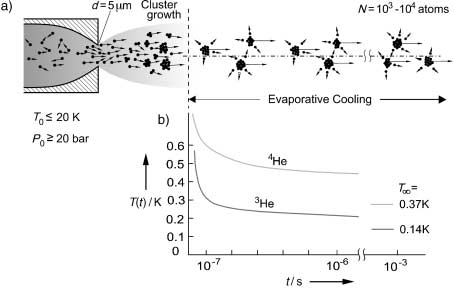
\includegraphics[width=0.6\textwidth]{../Images/jet_scketch.png}
	\caption[Scheme for a nozzle expansion]{ a) Schematic representation of the processes leading to the formation and subsequent cooling of helium droplets in a gas expansion. b) Calculated dependence of the droplet temperature on time for $^{4}He$ and $^{3}He$ droplets after they have left the cluster, taken from \cite{toennies_superfluid_2004}	}
	\label{img:jet}	
\end{figure}

\begin{figure}[h!]
\centering
	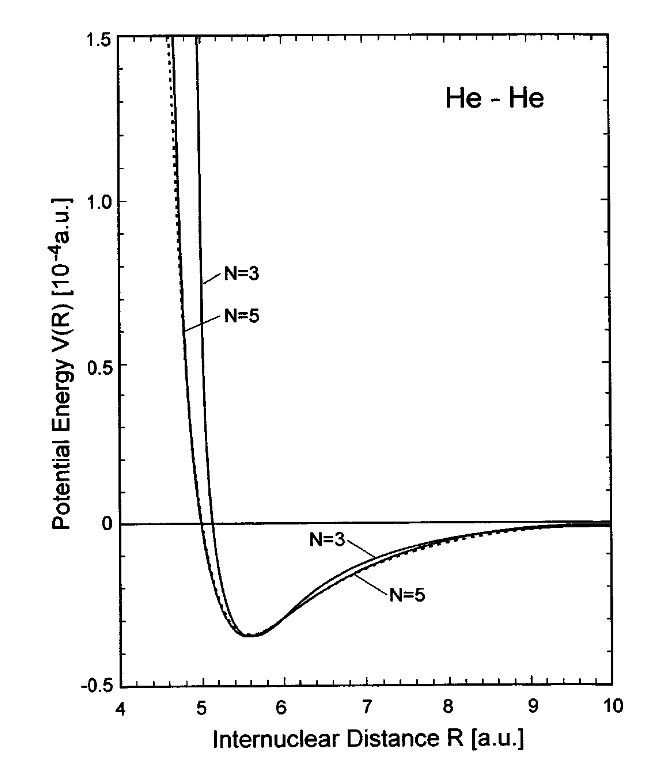
\includegraphics[width=0.5\textwidth]{../Images/waanderwaal_hehe.PNG}
	\caption[Waan der Wall He-He potential]{ Waan der Wals potential for He-He interaction}
	\label{img:WanderHe}
\end{figure}


When the Helium expands from the nozzel, its thermal energy is transform in kinetic energy of a supersonic flow field. After the expantion into the vacuum, the gas becomes supersaturated and condensations starts to occurs, creating the beam clusters. This clusters are made of atoms or moleulces held togueter by Wannder wals fores, in this case He-He interaction, that share the same kinetic vector. This means that the two particules travel as close and parallel to each other that a bonding is possible, see fig \ref{img:WanderHe}. From the reference frame of the cluster, each of its molecules are close to cero movments, in He this enhace the conditions to be liquid and in consecience superfluidity is achive  \cite{hagena_cluster_1972}.
 

There is no mathematical approach of the physics behind this cooling expansion but usually, Raleigh scattering measurements in combination with an empirical scaling law \cite{hagena_cluster_1972} are used to estimate the mean cluster size giving a certain degree of control over the cluster size distribution by adjusting the nozzle width and the source pressure. The droplet size distribution during supersonic expansion in the follows a log-normal distribution of the form \cite{harms_density_1998}.

\begin{equation}
p(N) = \frac{1}{\sqrt{2\pi}N \sigma} \exp  \left[- \frac{(ln(N/N_{0})^2}{2\sigma^2} \right]
\end{equation}
Where \textit{N} is the number of atom in the cluster, $\sigma$ is the distribution width and \textit{$N_{0}$} is the most likely numbers of atoms. Following it give a mean value.
\begin{align}
\bar N = \exp  \left(\mu+\frac{\sigma^2}{2} \right)
\end{align}
With a half width maxima of \cite{harms_density_1998}
\begin{align}
\sigma N_{\frac{1}{2}} = \exp \left( \mu - \sigma ^2 + \sigma \sqrt{2 ln(2)} \right) - \exp \left(  \mu - \sigma ^2 - \sigma \sqrt{2 ln(2)}  \right)
\end{align}

\begin{figure}[hbtp] \label{fig:ExpRegim}
\centering
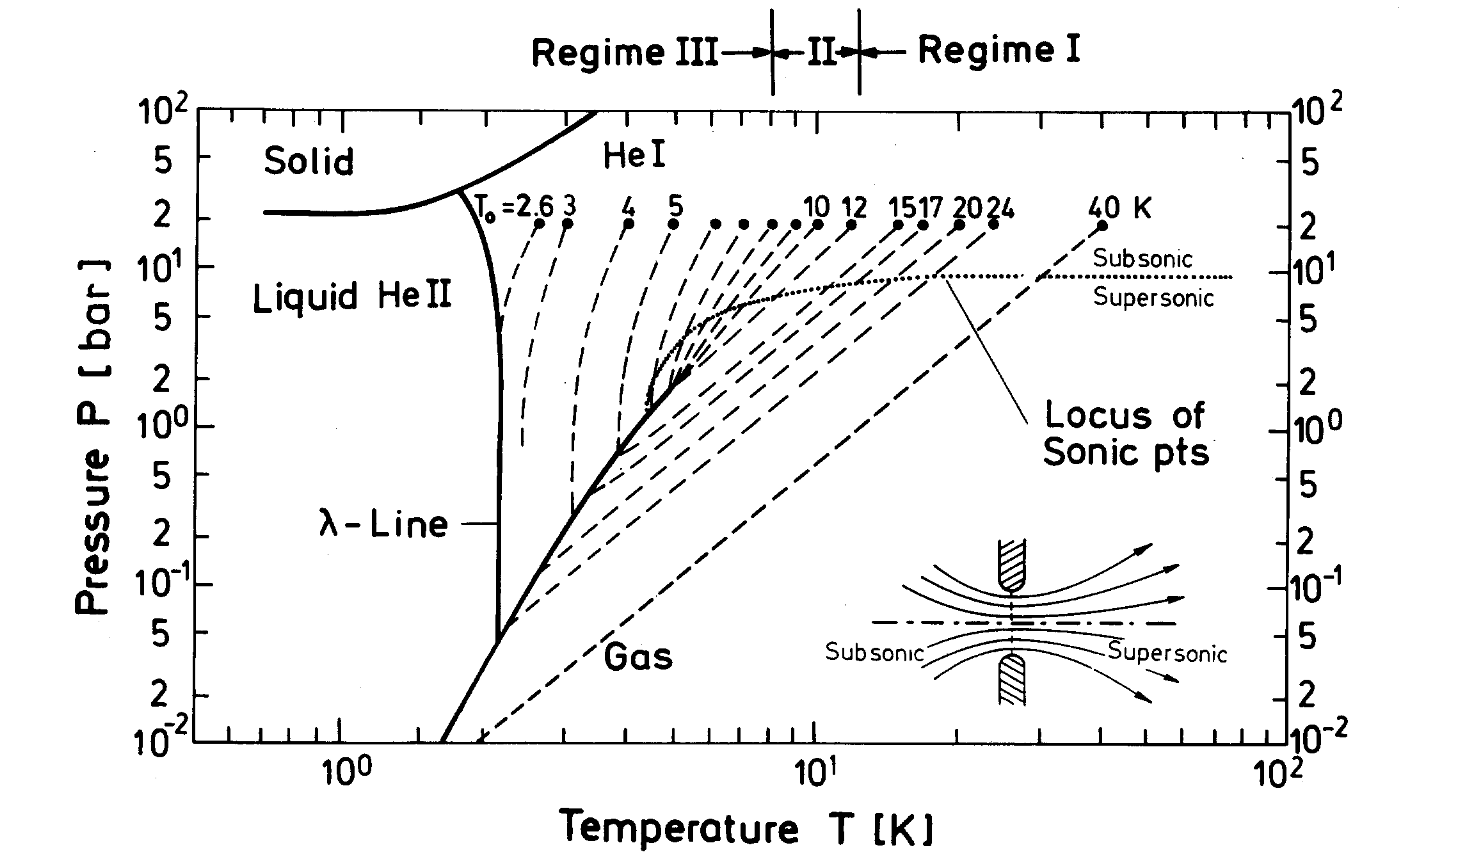
\includegraphics[width= 13 cm]{../Images/expansion_regimes.PNG}
\caption[Phase diagram for Expantion regimens]{Expansion regimes. Pressure-Temperatur phase diagram for $^{4}He$ for Nozzle beam expansions starting from a stagnation of 20 bar and a temperatures. As dicusse, quialitatively different behaivors are shown for the regime I - II and II where  starting in the gas phase,  near the phase trnasition respectivelly. taken from \cite{buchenau_mass_1990}. }
\end{figure}

As show in Figure \ref{fig:ExpRegim} The conditions in the He (pressure, temperature and nozzle size) in the free expansion will determine the characteristics of our final He beam. From Here three main regimes can be define.

Regime I or sub-critical expansion, begins in the gas phase and leads to droplet formation via condensation. this is the case of most expansions since the pressure are located below the critical pressure $P_{c}$.
Regime II, also called as critical expansion, is basically  and interminable regime that includes all trajectories which are near the critical point, leading to random expansion and difficult control of the beam due the large fluctuations in density.
Regime III, the  supercritical expansion, starts at low temperatures where the He stops behaving as an ideal gas, expecting flashing or cavitation  breaking up the liquid drops jet. \cite{buchenau_mass_1990}

super-critical and sub-critical regimes have been studies  in the last several years and  are clearly identified in the resulting size distributions. Figure \ref{img:dropletSize} shows that supercritical expansion forms large droplets (usually between $20-100 nm$ diameter) while a sub-critical expansion is suited to generate small droplets (around $5-10 nm$).  A simple relation that can be done to calculate the size or number of atom in a Custer is using. 

\begin{equation}
r=N_{1/3} * \rho A
\end{equation}

Where $r$ is the radius of the beam, $\rho$ is the density, in thhis case of He $\rho =0.0022 A $ \cite{stringari_systematics_1987}, but this approximation is not exact due the variation Of He density at this temperatures. As expected in both regimens for creating larger helium nano droplets, higher helium pressure and lower nozzle temperature are used. For our experiment a $5 \mu m$ nozzle was used at temperature oscillating between $11-15 K$, at pressure of $30 to 50$ bar.

\begin{figure}[hbtp]
\centering
\label{img:dropletSize}
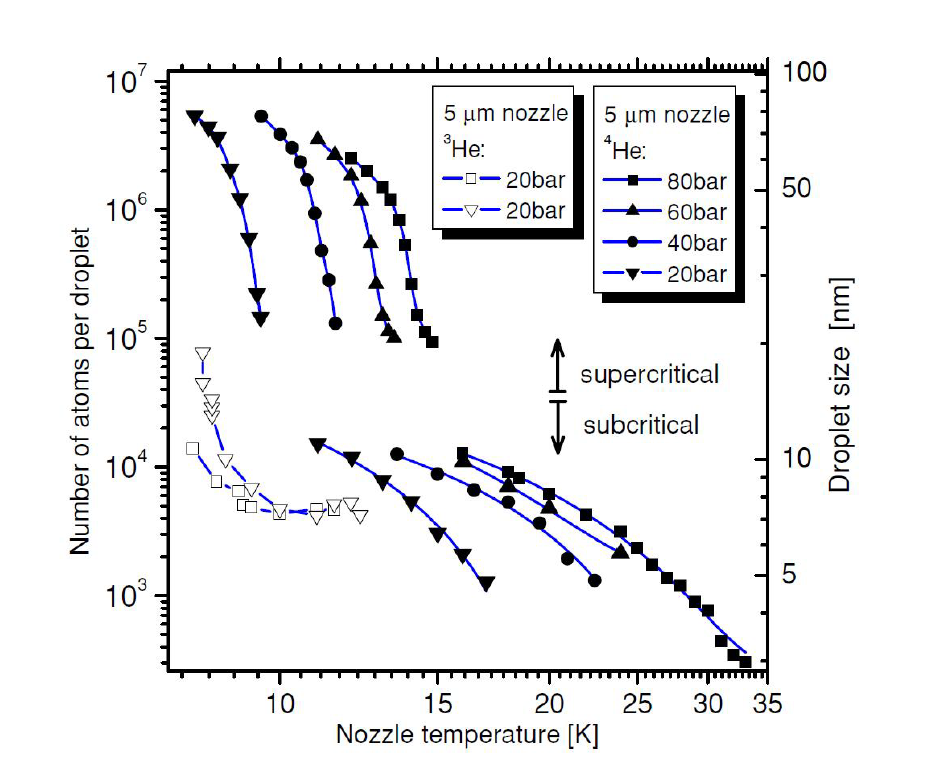
\includegraphics[scale=0.4]{../Images/sizes_regimen.PNG}
\caption[Expantion droplets Regimens]{Sizes of the $^{4}He$ droplets  as a function of nozzle temperature T and  pressures, based on \cite{toennies_spectroscopy_1998}, using a $5 \mu m$ nozzle. The su and super critical regimes are clearly diferenciated. Taken from \cite{stienkemeier_spsectroscopy_2006}}
\end{figure}


\subsubsection{Composite Clusters}

We can define a composite cluster or doped cluster, as a atom  bulk of one material that contains one or more different atomic elements. Usually in homogeneous clusters the main interest is their properties behaviour as a function of its size, but for doped clusters, the interaction between the elements creates new degrees of freedom that makes more complex its behaviour. For example, the new composite will have different structural properties due the spatial distribution of the species. Hence, composite clusters exhibit a more diverse behaviour and offer more opportunities to study different characteristics the material.

The first problem to overcome in composite cluster  is how to create them. Two techniques can be used. The first one, is the co expansion of
a previously mixed gas \cite{tchaplyguine_variable_2004} or the He cluster is produced first and then crossed with an atomic beam of the doping species.

The first technique  involves several technical problems, depends on possible interactions between the elements, the condensation ranges of the bulks and even in the  affinity  of the materials. One of the most used techniques, and the one used in this study is the one called pick-up technique \cite{gough_infrared_1985}. The idea is simple, as well as a snowball on its way downhill collects or pick-up more snow. The He cluster, after being directional selected through a Skimmer,  passes through a doping cell with a dopant gas at low densities ($10−2 Pa$) \cite{stienkemeier_spectroscopy_2006}. As a result, the gas atoms that are along the droplet cross sections will be captured by the beam and travel with it. The probability for helium droplets to collect $k$ atoms or molecules via inelastic collisions depends on the length of the oven cell $l$, the cross section of the droplets $\sigma$, and the particle density inside the cell $n$. As $l$ and $\sigma$ remains constant, varying the density in the doping cell can  regulated the abundance of $k$, following the Poissonian statistics:

\begin{equation}
P_{k}(l,n,\sigma)=\dfrac{(ln\sigma)^{k}}{k!} e^{(-ln\sigma)}
\end{equation}

Two important properties of these relation can be infer. First the maxima of different cluster sizes  are equidistant, $n_{max}=\dfrac{k}{l\sigma}$ and second, the exponential function in equation  becomes  nearly  one for  small  particle  densities \cite{bunermann_modeling_2011}.

Every pick-up process leads to an energy transfer to the droplets. As the dopant rapidly cool down to their, it means a transfer of energy to the He causing an  evaporaton of  helium atoms to keep the temperature unchanged. This He evaporation or "shrinkage", leads to a decrease of the cross section of the droplet and the probability to collect a further particle is  reduced. The involved energy is composed of the following contributions \cite{bunermann_modeling_2011}.

\begin{equation}
E=\langle E_{kin}\rangle + E_{in} + E_{binding} + E_{cluster}
\end{equation}

where

\begin{equation}
\langle E_{kin}\rangle \approx \dfrac{3}{2}k_{b}T + \dfrac{1}{2} m v^{2}
\end{equation}

is the kinetic energy of the droplet depending on it mass and velocity and temperature in the gas cell.

At a certain energy entry, the complete droplet evaporates if to may dopping acces to it. With $E_{kin}$ the average kinetic energy, $E_{in}$ the internal. Several studies have studied the $E_{binding}$ with $^{4}He$, given a broth number of materials to work with.. it also importat to take into acount that the binding energy include the cluste dopant binding as well as the dopant-dopant relation.\cite{toennies_spectroscopy_1998}. Acommung energy bounding for example $Xe-He$ is arround $26.9 meV$\cite{lewerenz_successive_1995}, or $He-H_{2}O$ is about $0.1 eV$ \cite{lewis_helium_2014}, AA more detailed table of all the energy bounding energy used in this study can be found in the appendix.

  
\section{Cluster-Intense Fields  Interaction}

To understanding of the interaction atoms-fields have been study broadly in physics since Einstein Photoionizasion Theory \cite{einstein_uber_1905}, that gives a base on all the quantum electrodynamics theory. The basics unders this theory is the behaivour of ligth as a electromagnetic field where the electron as a bounded charge in the atom can be afected.  This quantum dynamic theory is well understood since 1957 for small atoms, with one, two or few electrons \cite{a._bethe_quantum_1957}, but still big molecules and atoms have been challenging scientific for years. In this chapter we will give a brief introduction to the photoionization process, explaining at the same time multi-photoionization and tunnelling precesses, so we can finish with a more detailed presentation of Strong field interaction with clusters and the Keldish theory.


\subsection{PhotoIonization for single atoms}

The process of photoionization describes the leaving of an electron from its bound state  into the continuum by interaction with electromagnetic field radiation\cite{berkowitz_photoabsorption_1979}. The atomic bounded electrons while going through an electro magnetic field, in our case the laser beam,  can absorb enough  energy to get excited and fly away from the nucleus. A bound electron only can escape from an atom by absorbing photons its energy exceeds the binding energy of an electron \cite{einstein_uber_1905}. When the photon energy of the laser is smaller than the ionization potential of the target, the electron can absorb two or more photos in the ionization process, this is called Multi photon ionization (MPI). Another possible process is called, tunnelling ionization, where due the quantum mechanic properties of the electrons under certain conditions absorb enough energy enough to be on an above threshold regime and due it quantum dynamic properties it can escape from it bounds via tunnelling.

There is a variety of theoretical approaches to describe interaction of  laser fields with atoms. The Hamiltonian of the system of $N$ particles (ions and electrons) with pair-wise Coulomb interactions under the action of an external time-dependent electric field has the form:
\begin{equation}  \label{eq:hamiltonian}
\centering
H = \displaystyle\sum_{1 \leqslant i \leqslant N}^{} \dfrac{P_{i}}{2m_{i}} + \displaystyle\sum_{1 \leqslant i < j \leqslant N}^{} \dfrac{q_{i}q_{j}}{\mid r_{i}-r_{j} \mid} + \displaystyle\sum_{1 \leqslant i \leqslant N}^{n} q_{i}r_{i}\varepsilon(t)
\end{equation}

where $ r_{i,  p_{i}} $ and $ q_{i} $ are the coordinates, momenta and charge of the particles including the interaction between the classical electric field and $ \varepsilon(t) $ where \cite{mikaberidze_atomic_1981}

\begin{equation}
\varepsilon(t) = \varepsilon_{0} e_{z}cos(\omega t + \varphi)
\end{equation}

The proces that drives ionization can be divide on two regimes, a quantum electrical regime and a clasical one. \cite{karnakov_strong_2009}. Equation \ref{eq:hamiltonian}, use the non-relativistic approximation and neglect contributions from magnetic fields. The classical description of the laser field is a good approximation
for intense enough pulses, otherwise, quantum electrodynamics description is necessary.

An electron in the initial level with enery $E_{i}$ can absorb an photon with energy $\hbar \omega$ leading to final transition where $E_{f}-E_{i}=\hbar \omega$, when the enrgy of the photon is larger than the bounding energy, or the Ionization barrier the elctron is free with a the remainin kinetic energy $E_{kin} = \hbar \omega - I_{pot}$ \cite{becker_vuv_1996}.
In classical mechanics the probability of the energy transition depends directly on the cross section $(\sigma)$ of the electron in it was of the field However,  in  quantum  mechanics,  the photoionization cross section is related to the its transition probability between the initial and the final state given by Fermi’s golden rule

 \begin{equation} \label{eq:transitionprobability}
W_{|i\rangle \rightarrow |f\rangle} = \frac{2\pi}{\hbar\hbar} |\langle f|H|i\rangle|^{2} \delta(E_{i} - E_{f}-\hbar\omega)
 \end{equation}
 
 \begin{equation}\label{eq:crosssecQ}
 \sigma(\hbar\omega) = \dfrac{2\pi}{3} \alpha a_{0}_{2} \hbar\omega |\langle f|r_{n}|i\rangle|^{2}
 \end{equation}
 


When eq. \ref{eq:transitionprobability} is thee transition probability of one lectron to jump from minitial state $i$ to final state $f$, where $H$ is the hamiltonian operator. Eq. \ref{eq:crosssecQ} is the consequent cross sectiononsidering only the dipole part of the interaction Hamiltonian, where $\alpha$ is the fine structure coefficient, $r_{n}$ is the position operador of the electron $n$ \cite{fermi_quantum_1932}.

Energy photon needed to ionize an atom is directly proportional to the  the energetic distance between the electronic states and the ionization threshold. For  states closer to the ionization potential a  VUV photon can be enough to free a electron but for inner electrons  higher photon energies are required, varying from several tens eV to the order of several tens of keV, needing radiation sources at shorter wavelengths such as XUV to X-rays.\cite{becker_vuv_1996}

After photoionization is done, the electronic structure of the atom needs to rearrange via, due to the vacancy left by the ejected electron. Two relaxation processes can happens during this time. An electron from the outer shell will decay and replace the freed one, therefore the energy difference of the needs to be released in form of a fluorescence photon or Auger electron. On one hand, in case of a fluorescence decay the ionic state of the target does not change, since no additional electron is release. on the other hand, the Auger decay is a non radiative relaxation process, where a second electron is released from the Coulomb potential of the ion.

In example. as shown in fig.... if an photon  whit energy $\hbar\omega > E_{bin}$  ionized an electron, this will leave the atome lefting a gap. An electron in the higers level will replace the outer one, and lefting an ecxcess of energy. The outcome will be a fluerecence process with $E_{flu} = E_{in}- E_{out}$ or , the Auger $e-$, if $ E_{in}-E_{out} > E_{bond}$ and this electron can also escape the atomic Coulomb potential \cite{schmidt_electron_1997}.

\begin{figure}[hbtp] \label{fig:augerfluorec}
\centering
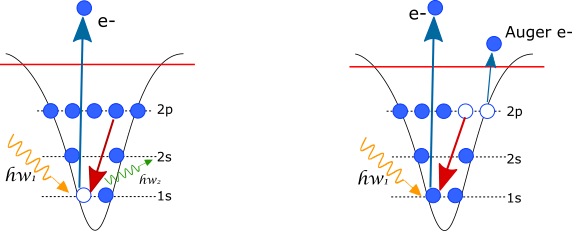
\includegraphics[width=6 cm]{../Images/text6418.png}
\caption[Relaxation processes for photoionization]{two example os the relaxation processes. On the left, A photon ionized an electron and the Electron Ein replaced, expelin a fluerecent photon in the process. on the rigth, the energie reliessed by the replacement electron is enougth to make another electron in the outer shell to also go to the continium, ASuger electron. taked form \cite{rafipoor_two-color_2017}}
\end{figure}

\subsection{Multhiphoton and tunelling Ionization}

Ionization is also possible even if one photon energy is lower than the binding potential. Electri field of lasers with intensities below $I \leqslant 10^{14}W/cm^{2}$ is not strong enougth to change the binding potzential of a atom significantly \cite{rhodes_multiphoton_1985}.  Multiphoton ionization (MPI is the simultaneous absorption of several photons to overcome the ionization barrier. The way MPI occurs in atoms depends on the laser frequency and intensity. When the intensity is much lower than the characteristic atomic resonance, MPI occurs via transitions through virtual states. Ionization by several photons at low laser intensities can be realized by the so-called resonance enhanced multiphoton ionization (REMPI)\cite{mainfray_multiphoton_nodate}.  Ionization by a REMPI process takes place in two steps
In the first step, a resonant excitation by one or more photons takes place on an electron state of the atom. In the second step, this electron state is transformed into a virtual state, to a state until the electron is excited by spontaneous decay. So for example the total energy absirbed by an electon until it gets ionizes is $n * \hbar\omega > I_{pot}$ where $n$ is the number of photon absorbes until it actially have enougth energy to overcome the potencial $I_{pot}$

For Laser intensities $I > 10^{14}W/cm^{2}$, higher intensities and lower frequencies, tunneling ionization (TI) is more likely to occur.  In this case, thebinding potential of the atom get is strongllöy afected by the electric fiels of the laser. Arround the peack of the electri field the  potential gets narrower, and the elctron in the outer states get closest to the bidding barrier. allowing the electron to tunneling througth the confining potential into de contzinium\cite{griffiths_introduction_2013}. TI is inherently a quantum process. The bending of the Coulomb potential becomes by the supperpossition of the coulomb potential and the laser field. Therefore TI must occure when the time of the ionization is shorter thatan a laser oscilation cycle\cite{berkowitz_photoabsorption_1979}. Based in the same principle, when the Laser fiel becomes so strong to lower the binding potencial that separates the highest electron level, then the electrons in this state become free electrons. This process is called barrier suppression Ionisattopn or BSI\cite{krishnan_doped_2011}.

In the fig \ref{img:ionizationprocess}, we present a scketch of the 3 possible ionization processes explained above. On the lefte we present an simple ionization process where a photon with energy $E_{phot} = \hbar\omega$ is higher than the potential barrier. In the center a MPI process is shown, $n$ photons exite the inner-shell electron, exiting it througth virtual level until it finally have enougth energy to be free to the continium. Finally on the left a TI happens. Here the coulomb potencia barrier is afectis by the laser files bending ii, The outter shell electron  gets closets to it and via tunneling  can get ionize\cite{rafipoor_two-color_2017}.

\begin{figure}[hbtp]
\label{img:ionizationprocess}
\centering
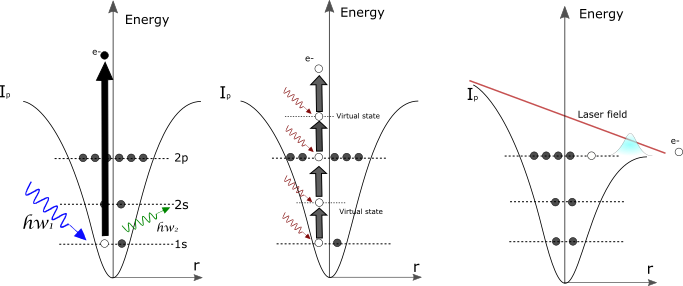
\includegraphics[width = 8 cm]{../Images/photoionization2.png}
\caption[Ionization regimes]{ On the left is the scketch of a single photon ionization process, where a photon with energy $E_{phot} = \hbar\omega$ is higher than the potential barrier $I_{p}$. On the center the MPI process,  inner-shell electron absorbs $n$ photons, getting excited througth the electronic levels (reals or virtual)  until it reach the continium. On the left the BSI Process, the coulomb potencial barrier bends by the laser fields, been lower than the outer shell electron state, the electrons can scape easilly. based on \cite{rafipoor_two-color_2017}.}
\end{figure}


As explained the Intensity of the external fiel plays an important rol in the ionizaion process. A brather eazzy whay to differenciate when each process needs to be taken into account is provides by the Keldysh parameter\cite{keldysh_ionization_1965}.

\begin{equation}
\gamma_{k}=\sqrt{\dfrac{I_{p}}{2U_{p}}}
\end{equation}

Where $\gamma_{k}$ is the Keldish parameter, $I_{p}$ is the atoms ionization potential and $U_{p}$ is the ponderomotive potential defined as

\begin{equation}
U_{p} = \dfrac{e^{2}E_{0}^{2}}{4m_{e}\omega_{0}^{2}} \propto I \lambda^{2}
\end{equation}

where $m_{e}$ is the mass of the electron, $\omega_{0}, \lambda, I$ and $E_{0}$ are the frecuency, wavelengst, intensity and the peak of the electric field of the laser pulse. On one hand, when the Keldish parameter is higher, $\gamma_{k} \gg 1$ MPI regime is conside. on the other hand, the $\gamma_{k} \ll 1$ describes the TI interaction.








